
%%%%%%%%%%%%%%%%%%%%%%%%%%%%%%%%%%%%%%%%%%%%%%%%%%%%%%%%%%%%%%%%%%%%
\section{Architecture\label{sec:kds_architecture}}

%%%%%%%%%%%%%%%%%%%%%%%%%%%%%%%%%%%%%%%%%%%%%%%%%%%%%%%%%%%%%%%%%%%%

This package provides a framework to allow exact implementation of
kinetic data structures and sweepline algorithms. Below we discuss in
detail each one of the first four major concepts which help in
implementing kinetic data structures: the \ccc{Kinetic::Simulator},
the \ccc{Kinetic::Kernel}, the \ccc{Kinetic::ActiveObjectsTable} and the
\ccc{Kinetic::InstantaneousKernel}.  The \ccc{Kinetic::FunctionKernel}
concept is discussed separately in Section
\ref{sec:kds_algebraic_kernel}.

\begin{figure}
\begin{ccTexOnly}
\begin{center}
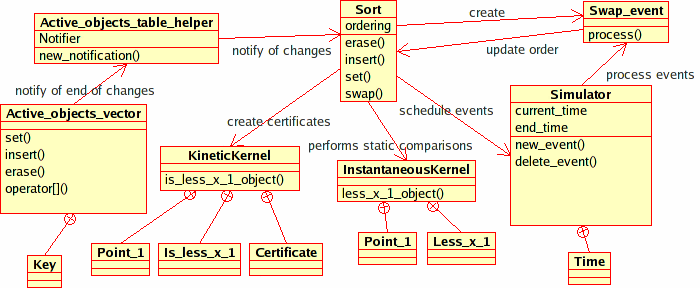
\includegraphics[scale=.8,viewport=0 18 470 250, clip]{Kinetic_data_structures/sort_usage_pct}
\end{center}
\end{ccTexOnly}
\begin{ccHtmlOnly}
<img src="./sort_usage_pct.gif" align=middle alt="Sort Usage"><br>
\end{ccHtmlOnly}
\caption{\label{fig:kds_uml_usage_architecture} The figure, identical
  to the one in the overview of the previous chapter, shows the
  interaction between the \ccc{Kinetic::Sort<Traits, Visitor>} kinetic
  data structure and the various pieces of our framework.  Other, more
  complicated, kinetic data structures will also use the
  \ccc{Kinetic::InstantaneousKernel} in order to insert/remove
  geometric primitives and audit themselves.
  \ccc{Kinetic::Sort<Traits, Visitor>} uses the sorting functionality
  in STL instead.}
\end{figure}

\subsection{The Kinetic::Simulator\label{sec:kds_simulator}}


The \ccc{Kinetic::Simulator} is the central repository of all active events.
It maintains the event queue and can use its knowledge of the events
in the queue to find times for the kinetic data structures to easily
check their own correctness (this will be discussed in more detail
later in this section). Kinetic data structures call methods of the
\ccc{Kinetic::Simulator} to schedule new events, deschedule old ones and
access and change data contained in already scheduled events (the
operations on existing events are performed using a key which was
returned when the event was scheduled).  For controlling the
simulation, methods in the \ccc{Kinetic::Simulator} allow stepping through
events, advancing time and even running the simulation backwards (that
is we run the simulation with the time running in the opposite
direction).

The kinetic sorting example in Figure~\ref{sec:kds_sort_example} shows the
basic usage of the \ccc{Kinetic::Simulator}. First, the \ccc{Simulator}
is created by the \ccc{Kinetic::SimulationTraits}. The kinetic data structure
gets a handle to the simulator from the traits class and uses the
handle to add its events to the simulation. The \ccc{Kinetic::Simulator} is
then told to advance time up until the end of the simulation,
processing all events along the way.

Each event is represented by a \ccc{Kinetic::Simulator::Time} and an instance of a
model of the \ccc{Kinetic::Simulator::Event} concept.  Models of the \ccc{Kinetic::Simulator::Event}
concept are responsible for taking the appropriate action in order to
handle the kinetic event they represent.  Specifically, the
\ccc{Kinetic::Simulator::Event} concept specifies one method,
\ccc{Kinetic::Simulator::Event::process()}, that is called when the event occurs.
The body of the \ccc{Kinetic::Simulator::Event::process()} method typically
simply calls a method of the kinetic data structure that created the
event; for example in our kinetic sorting example, processing an event
means calling the \ccc{Kinetic::Sort<Traits, Visitor>::swap(Iterator)}
method of the kinetic sorting data structure.

In the model of the \ccc{Kinetic::Simulator} concept that we provide,
\ccc{Kinetic:Default_simulator<FunctionKernel, EventQueue>}, any model
of the \ccc{Kinetic::Simulator::Event} concept can be inserted as an
event. This ability implies that events can be mixed at run time,
which is essential when we want to support multiple kinetic data
structures operating on the same set of moving geometric primitives.

The \ccc{Kinetic::Simulator::Time} concept is defined by the simulator, typically to be
some representation of a root of a polynomial, taken from the
\ccc{Kinetic::FunctionKernel} (details of the algebraic side of the package
will be discussed in Section~\ref{sec:kds_algebraic_kernel}). For most
kinetic data structures \ccc{Kinetic::Simulator::Time} only needs to support
comparisons (we need to compare events, in order to process them in
the correct order) and a few other non-arithmetic operations.

When the failure times of certificates are sorted exactly (as opposed
to when we numerically approximate the roots of the certificate
polynomials) the correctness of kinetic data structures can be easily
verified.  Let $I$ be an open interval between the last event
processed and the next event to be processed.  As was mentioned in the
introduction kinetic data structures do not change combinatorially in
$I$. In addition, although the static data structures can be
degenerate at the roots defining the two ends of the interval, they
are not, in general, degenerate in the interior. An independent check
of the integrity of kinetic data structures can be provided by, for
example, using an \ccc{Kinetic::InstantaneousKernel} (cf. Subsection
\ref{sec:kds_instantaneous_kernel}) to rebuild the static version of the
structure from scratch at some time interior to $I$ and compare it to
the kinetic version. This auditing can typically catch algorithmic or
programming errors much closer to the time they arise in the
simulation than, for example, using visual inspection.  Such easy
auditing is one of the powerful advantages of having an exact
computational framework since, as with static data structures, when
using inexact computations differentiating between errors of
implementation and numeric errors is quite tricky.

Kinetic data structures receive alerts of appropriate times to audit
themselves using a notification framework. The same framework is also
used by the \ccc{Kinetic::ActiveObjectsTable} to alert kinetic data
structures when the set of primitives changes (see
Subsection~\ref{sec:kds_active_objects_table}). To use the notification
framework, the kinetic data structure creates a proxy object which
implements a standard \ccc{Listener} interface. It then registers this
proxy with the \ccc{Kinetic::Simulator}. When the
\ccc{Kinetic::Simulator} finds an appropriate time for the kinetic
data structures to audit themselves it calls the function
\ccc{Listener::new_notification(Type)} on each of the registered proxy
objects.  A helper for creating such proxy objects, called
\ccc{Kinetic::Simulator_kds_listener<Listener, KDS>}, is provided by the
framework. It translates the notification into a function call
(\ccc{audit()}) on the kinetic data structure.  Pointers in the
notification framework are reference counted appropriately to avoid
issues caused by the creation and destruction order of kinetic data
structures and the simulator. See Section~\ref{sec:kds_listener} for a more
complete discussion of this part of the framework.

Internally the \ccc{Kinetic::Simulator} maintains a priority queue
containing the scheduled events. The type of the priority queue is a
template argument to our \ccc{Kinetic::Simulator} model and, as such, it can
be replaced by the user.  In our package, we provide two different
types of priority queues, a heap and a two-list priority queue.  A
two-list queue is a queue in which there is a sorted front list,
containing all events before some time and an unsorted back list. The
queue tries to maintain a small number of elements in the front list,
leaving most of them in the unsorted main pool. The two-list queue,
although an unconventional choice, is our default queue when using
exact computation because it minimizes comparisons involving events
that are far in the future.  These events are likely to be deleted
before they are processed, so extra work done structuring them is
wasted.  Our experiments have shown that, for example, the two-list
queue causes a 20\% reduction in running time relative to a binary
heap for Delaunay triangulations with degree 3 polynomial motions and
20 points.



\subsection{The Kinetic::Kernel}

The \ccc{Kinetic::Kernel} is structured very much like static CGAL
kernels. It defines a number of primitives, which in the model
provided are \ccc{Kinetic::Kernel::Point_1},
\ccc{Kinetic::Kernel::Point_2}, \ccc{Kinetic::Kernel::Point_3} and
\ccc{Kinetic::Kernel::Weighted_point_3}. The primitives are defined by
a set of Cartesian coordinates each of which is a function of time, a
\ccc{Kernel::MotionFunction}. In addition it defines constructions
and certificate generators which act on the primitives.  The
certificate generators are the direct analog of the non-kinetic
predicates. Each certificate generator take a number of primitives as
arguments, but instead of producing an element from a discrete set
they produce a set of discrete failure times for the certificate.
These failure times are wrapped in a model of \ccc{Kinetic::Certificate}.

A \ccc{Kinetic::Certificate} is a simple object whose primary function is to
produce a \ccc{Kinetic::Simulator::Time} object representing the failure time of the
certificate.  Since, the handling of most certificate failures
involves creating a new certificate whose certificate function is the
negation of the old certificate function, a \ccc{Kinetic::Certificate}
object caches any work that could be useful to isolate future roots of
the certificate function (such as the Sturm sequence of the
certificate function). To illustrate this further, if you have two
one-dimensional points with coordinate functions $p_0(t)$ and
$p_1(t)$, the certificate that the first moving point is after the
second corresponds to the inequality $p_0(t) - p_1(t) > 0$.  When the
certificate fails and the two points cross, the new certificate is
$p_1(t)- p_0(t) > 0$, which is the negated version of the certificate
just processed and which has the same roots.

The model of \ccc{Kinetic::Kernel} provided includes the certificate
generators necessary for Delaunay triangulations (in one, two and
three dimensions) and regular triangulations (in 3D).  New
certificates can be fairly easily added. An example is included in the
distributed code.



\subsection{The Kinetic::ActiveObjectsTable\label{sec:kds_active_objects_table}}


The \ccc{Kinetic::ActiveObjectsTable} stores a set of kinetic primitives.
Its purpose is to notify kinetic data structures when new primitives
are added, when primitives are removed or when a trajectories change.
Each primitive is uniquely identified by a Key, assigned by
the table when the primitive is added, that can be used to change or
remove it.  We provide one model of the
\ccc{Kinetic::ActiveObjectsTable} concept, called
\ccc{Kinetic::Active_objects_vector<MovingObject>} which stores all the moving
primitives in an \ccc{std::vector<D>}.

Notifications of changes to the set of active objects are handled
using a setup similar to the \ccc{Kinetic::Simulator} audit time
notification. We provide a helper class,
\ccc{Kinetic::Active_objects_listener_helper<ActiveObjectsTable,
KDS>}, which translates the notifications into \ccc{insert(Key)},
\ccc{erase(Key)} or \ccc{set(Key)} function calls on the kinetic data
structure.



\subsection{The Kinetic::InstantaneousKernel\label{sec:kds_instantaneous_kernel}}


The \ccc{Kinetic::InstantaneousKernel} allows existing \cgal\ data structures
to be used on moving data as it appears at some instant of time.
Models of this concept are, by definition, models of a CGAL
Kernel or a traits class, and, therefore, can then be used as
the traits class of CGAL's algorithms and data structures.

Consider for example the kinetic Delaunay data structure in either two
or three dimensions.  Internally, it uses a
\ccc{Delaunay_triangulation_2<Traits, Tds>} or
\ccc{Delaunay_triangulation_3<Traits, Tds>} to represent the
triangulation, instantiated with a model of the
\ccc{Kinetic::InstantaneousKernel} concept as its traits class.  At
initialization, as well as at times during the simulation when we want
to insert a point to the kinetic Delaunay triangulation, a static
version of the Delaunay triangulation is conceptually instantiated.
More precisely, the time for the copy of the model of the
\ccc{Kinetic::InstantaneousKernel} stored in the \cgal\ triangulation is set
to be the current time (or rather, as discussed in the introduction, a
more convenient time determined by the \ccc{Kinetic::Simulator}
combinatorially equivalent to the current time).  The kinetic data
structure then calls the
\ccc{Delaunay_triangulation_3<Traits, Tds>::insert(Point)} insert
method to insert the point.  The static insert method called uses
various predicate functors on the moving points which evaluate to the
values that the predicates have at that instant in time. Removal is
handled in an analogous manner. Auditing of the geometric structure is
easily handled in a similar manner (in the case of Delaunay
triangulations by simply calling the \ccc{verify()} method after
setting the time).

%%%%%%%%%%%%%%%%%%%%%%%%%%%%%%%%%%%%%%%%%%%%%%%%%%%%%%%%%%%%%%%%%%%%
\subsection{Miscellaneous: notification and reference management\label{sec:kds_misc}}

%%%%%%%%%%%%%%%%%%%%%%%%%%%%%%%%%%%%%%%%%%%%%%%%%%%%%%%%%%%%%%%%%%%%

We describe some coding conventions used, graphical display,
notification and reference management support in the framework in the
following sections.


\subsubsection{Reference management}

A number of objects need to maintain pointers to other independent
objects. For example, each kinetic data structure must have access to
the \ccc{Kinetic::Simulator} so that it can schedule and deschedule
events. These pointers are all reference counted in order to guarantee
that they are always valid. We provide a standard reference counting
pointer and object base to facilitate this, namely
\ccc{Ref_counted<Object>}.

Each shared object in the framework defines a type \ccc{Handle} which is the
type for a reference counter pointer pointing to it. These should be
used for storing pointers to the objects in order to avoid dangling
pointers. In addition, many of the objects expect such pointers as
arguments.

\subsubsection{Runtime event passing\label{sec:kds_listener}}


Runtime events must be passed from \textit{notifiers}, namely the
\ccc{Kinetic::ActiveObjectsTable} and the \ccc{Kinetic::Simulator} to
\textit{listeners}, typically the kinetic data structures. For
example, kinetic data structures are notified when new primitives are
added to the \ccc{Kinetic::ActiveObjectsTable}. On reciving the
notification, it will add the new primitive to the combinatorial
structure it is maintaining. The events are passed using a simple,
standardized notification interface. To receive notifications, the
listener first defines a small proxy class which inherits from a
\ccc{Listener} base type provided by the notifier. On creation, the
\ccc{Listener} base class registers itself with the notifier on
construction (and unregisters itself on destruction).

When the some state of the notifier changes, it calls the
\ccc{new_notification} method on the listener proxy object provided
and passes it a label corresponding to the name of the field that
changed. The proxy object can then call an appropriate method on the
kinetic data structure or whetever the listening class is.

In order to unregister on destruction, the \ccc{Listener} must store a
(reference counted) pointer to the object providing notifications.
This pointer can be accessed through the \ccc{notifier()} field. The
\ccc{Listener} object stores a reference counted pointer to the
notifying object, while the notifying object stores a plain pointer to
the \ccc{Listener}. It can do this since the \ccc{Listener} is
guaranteed to unregister itself when it is destroyed. This avoids
circular reference counted pointers as well as dangling pointers.

\section{Algebraic Kernel\label{sec:kds_algebraic_kernel}}


The interface between the algebraic kernel and the kinetic data
structures package was kept quite minimal in order to ease the
implementation of various underlying computation models. The interface
is detailed in the reference page (\ccc{Kinetic::FunctionKernel}).

We provide models of the algebraic kernel that handle polynomial
\ccc{Kinetic::Function} objects. The provided models perform
\begin{itemize}
\item exact computations using Sturm sequences to isolate roots
\item exact computations using Descartes rule of sign in order to
  isolate roots (Sturm sequences are also used in order to properly
  handle even multiplicity roots)
\item filtered exact computations using Descartes rule of sign
\item numeric (inexact) root approximations
\item numeric root approximations which take advantage of certain
  assumptions that can be made about the types of polynomials solved
  in the process of evaluating kinetic data structures
\item a wrapper for CORE::Expr which implements the required
  concepts.
\end{itemize}
The exact models, which we implement the numerics for, handle
non-square-free polynomials and polynomials with arbitrary field
number type coefficients and are quite robust.


\subsection{Kinetic::FunctionKernel customized for kinetic data structures}

There are several modifications we can make to how the roots are
handled to optimize for the case of kinetic data structures.  The
first are motivated by the question of how to handle degeneracies
(certificate functions which have roots at the same time).  Naively,
there is no way to differentiate between a certificate which fails
immediately when it is created and one whose function is momentarily
0, but will be valid immediately in the future. In order to handle
such degeneracies we ensure that all the certificate function
generators produce certificate functions which are positive when the
corresponding certificates are valid.  Then, if we have a degeneracy
we can differentiate between a certificate which fails immediately and
one which is simply degenerate by looking at the sign of the
certificate function immediately following the root (equivalently, by
looking at the derivative). In addition, this allows us, under the
assumption that computations are performed exactly, to check that all
certificates are not invalid upon creation.

The assumption that certificates are positive when valid is particular
useful when using numeric solvers.  Without it there is no reliable
way to tell whether a root near the current time is the certificate
having become valid just before the current time, or failing shortly
in the future. Testing the sign of the function immediately after the
root reliably disambiguates the two cases.

In addition, we have to specially handle even roots of functions. For
the most part these can just be discarded as dropping an even root is
equivalent to perturbing the simulation to remove the degeneracy.
However, when we are using the \ccc{Kinetic::Simulator} to audit the
kinetic data structures, they most be broken up in to two, equal,
roots to avoid auditing at the degeneracy.
